\chapter{Detailed System Design}

\section{Detailed System Architecture}

\subsection{Microservices Architecture Overview}

Deploying a complex medical annotation system in healthcare environments presents significant challenges that necessitate a microservices architecture approach \cite{newman2015building}. Traditional monolithic systems that bundle all functionality into a single application create operational bottlenecks and deployment complexities that are particularly problematic in medical imaging workflows where reliability, scalability, and integration flexibility are critical.

\textbf{Critical Need for Microservices Architecture:} Medical annotation systems must address diverse institutional requirements where different healthcare facilities have varying levels of technical infrastructure, IT expertise, and computational resources. The heterogeneous nature of medical imaging environments demands an architecture that can optimize resource utilization while maintaining system reliability. A microservices approach becomes essential to enable:

\begin{itemize}
    \item \textbf{Optimized Resource Allocation:} Deploy only necessary components, dramatically reducing hardware requirements and operational costs while maintaining full functionality
    \item \textbf{Dynamic Scaling Capability:} Scale individual services independently based on real-time demand patterns (e.g., additional viewer instances during peak annotation periods, expanded AI processing during batch operations)
    \item \textbf{Zero-Downtime Maintenance:} Update, patch, or maintain services independently without disrupting ongoing annotation workflows, ensuring continuous availability for critical medical operations
    \item \textbf{Seamless Legacy Integration:} Integrate with existing hospital information systems through standardized APIs without requiring wholesale infrastructure replacement
    \item \textbf{Fault Isolation and Recovery:} Handle component failures gracefully with automatic failover capabilities, preventing single points of failure from compromising entire annotation workflows
    \item \textbf{Performance Optimization:} Optimize each service for its specific computational requirements (e.g., GPU acceleration for AI services, high-throughput storage for DICOM data)
\end{itemize}

\textbf{Strategic Service Decomposition:} The architecture is strategically decomposed into four specialized services, each optimized for specific functional domains and performance characteristics:

\begin{itemize}
    \item \textbf{Workflow Management Service (latn-5):} React-based platform using Supabase for real-time collaboration, handling project creation, task assignment, user management, and workflow orchestration
    \item \textbf{Annotation Interface Service (latn-3-ohif3):} Enhanced OHIF Viewer providing medical image visualization, annotation tools, AI integration, and collaborative features
    \item \textbf{AI Assistance Service (MONAI Label):} Containerized AI engine delivering foundation model support, interactive segmentation, and model-in-the-loop learning capabilities
    \item \textbf{Data Management Service (Orthanc PACS):} DICOM-compliant storage system managing medical image storage, metadata indexing, and integration with existing hospital PACS infrastructure
\end{itemize}

\textbf{Intelligent Communication Architecture:} Services communicate through optimized API patterns that minimize latency and maximize throughput in medical imaging workflows. The system implements smart caching, connection pooling, and request batching to ensure optimal performance. For instance, when a user opens a medical study, the system orchestrates parallel data retrieval from multiple services while prefetching likely-needed resources, resulting in significantly faster load times and improved user experience.

\textbf{Adaptive Deployment Optimization:} The microservices architecture enables deployment strategies that can be precisely matched to available infrastructure and performance requirements. This flexibility allows for optimization ranging from lightweight containerized deployments for resource-constrained environments to distributed cloud-native deployments that can scale dynamically based on demand, ensuring optimal performance-to-cost ratios across diverse operational scenarios.

\textbf{Continuous Performance Enhancement:} The modular nature enables targeted optimization of individual components without affecting the entire system. This allows for iterative performance improvements, technology stack upgrades, and feature enhancements while maintaining system stability and backward compatibility, ensuring the annotation platform can evolve with advancing medical imaging requirements and technological innovations.

Figure 4.1 illustrates the complete system architecture, demonstrating the end-to-end flow of the intelligent medical annotation system from user access through various integrated services, highlighting how the microservices architecture enables scalable, maintainable, and fault-tolerant medical imaging workflows.

\begin{figure}[htbp]
\centering
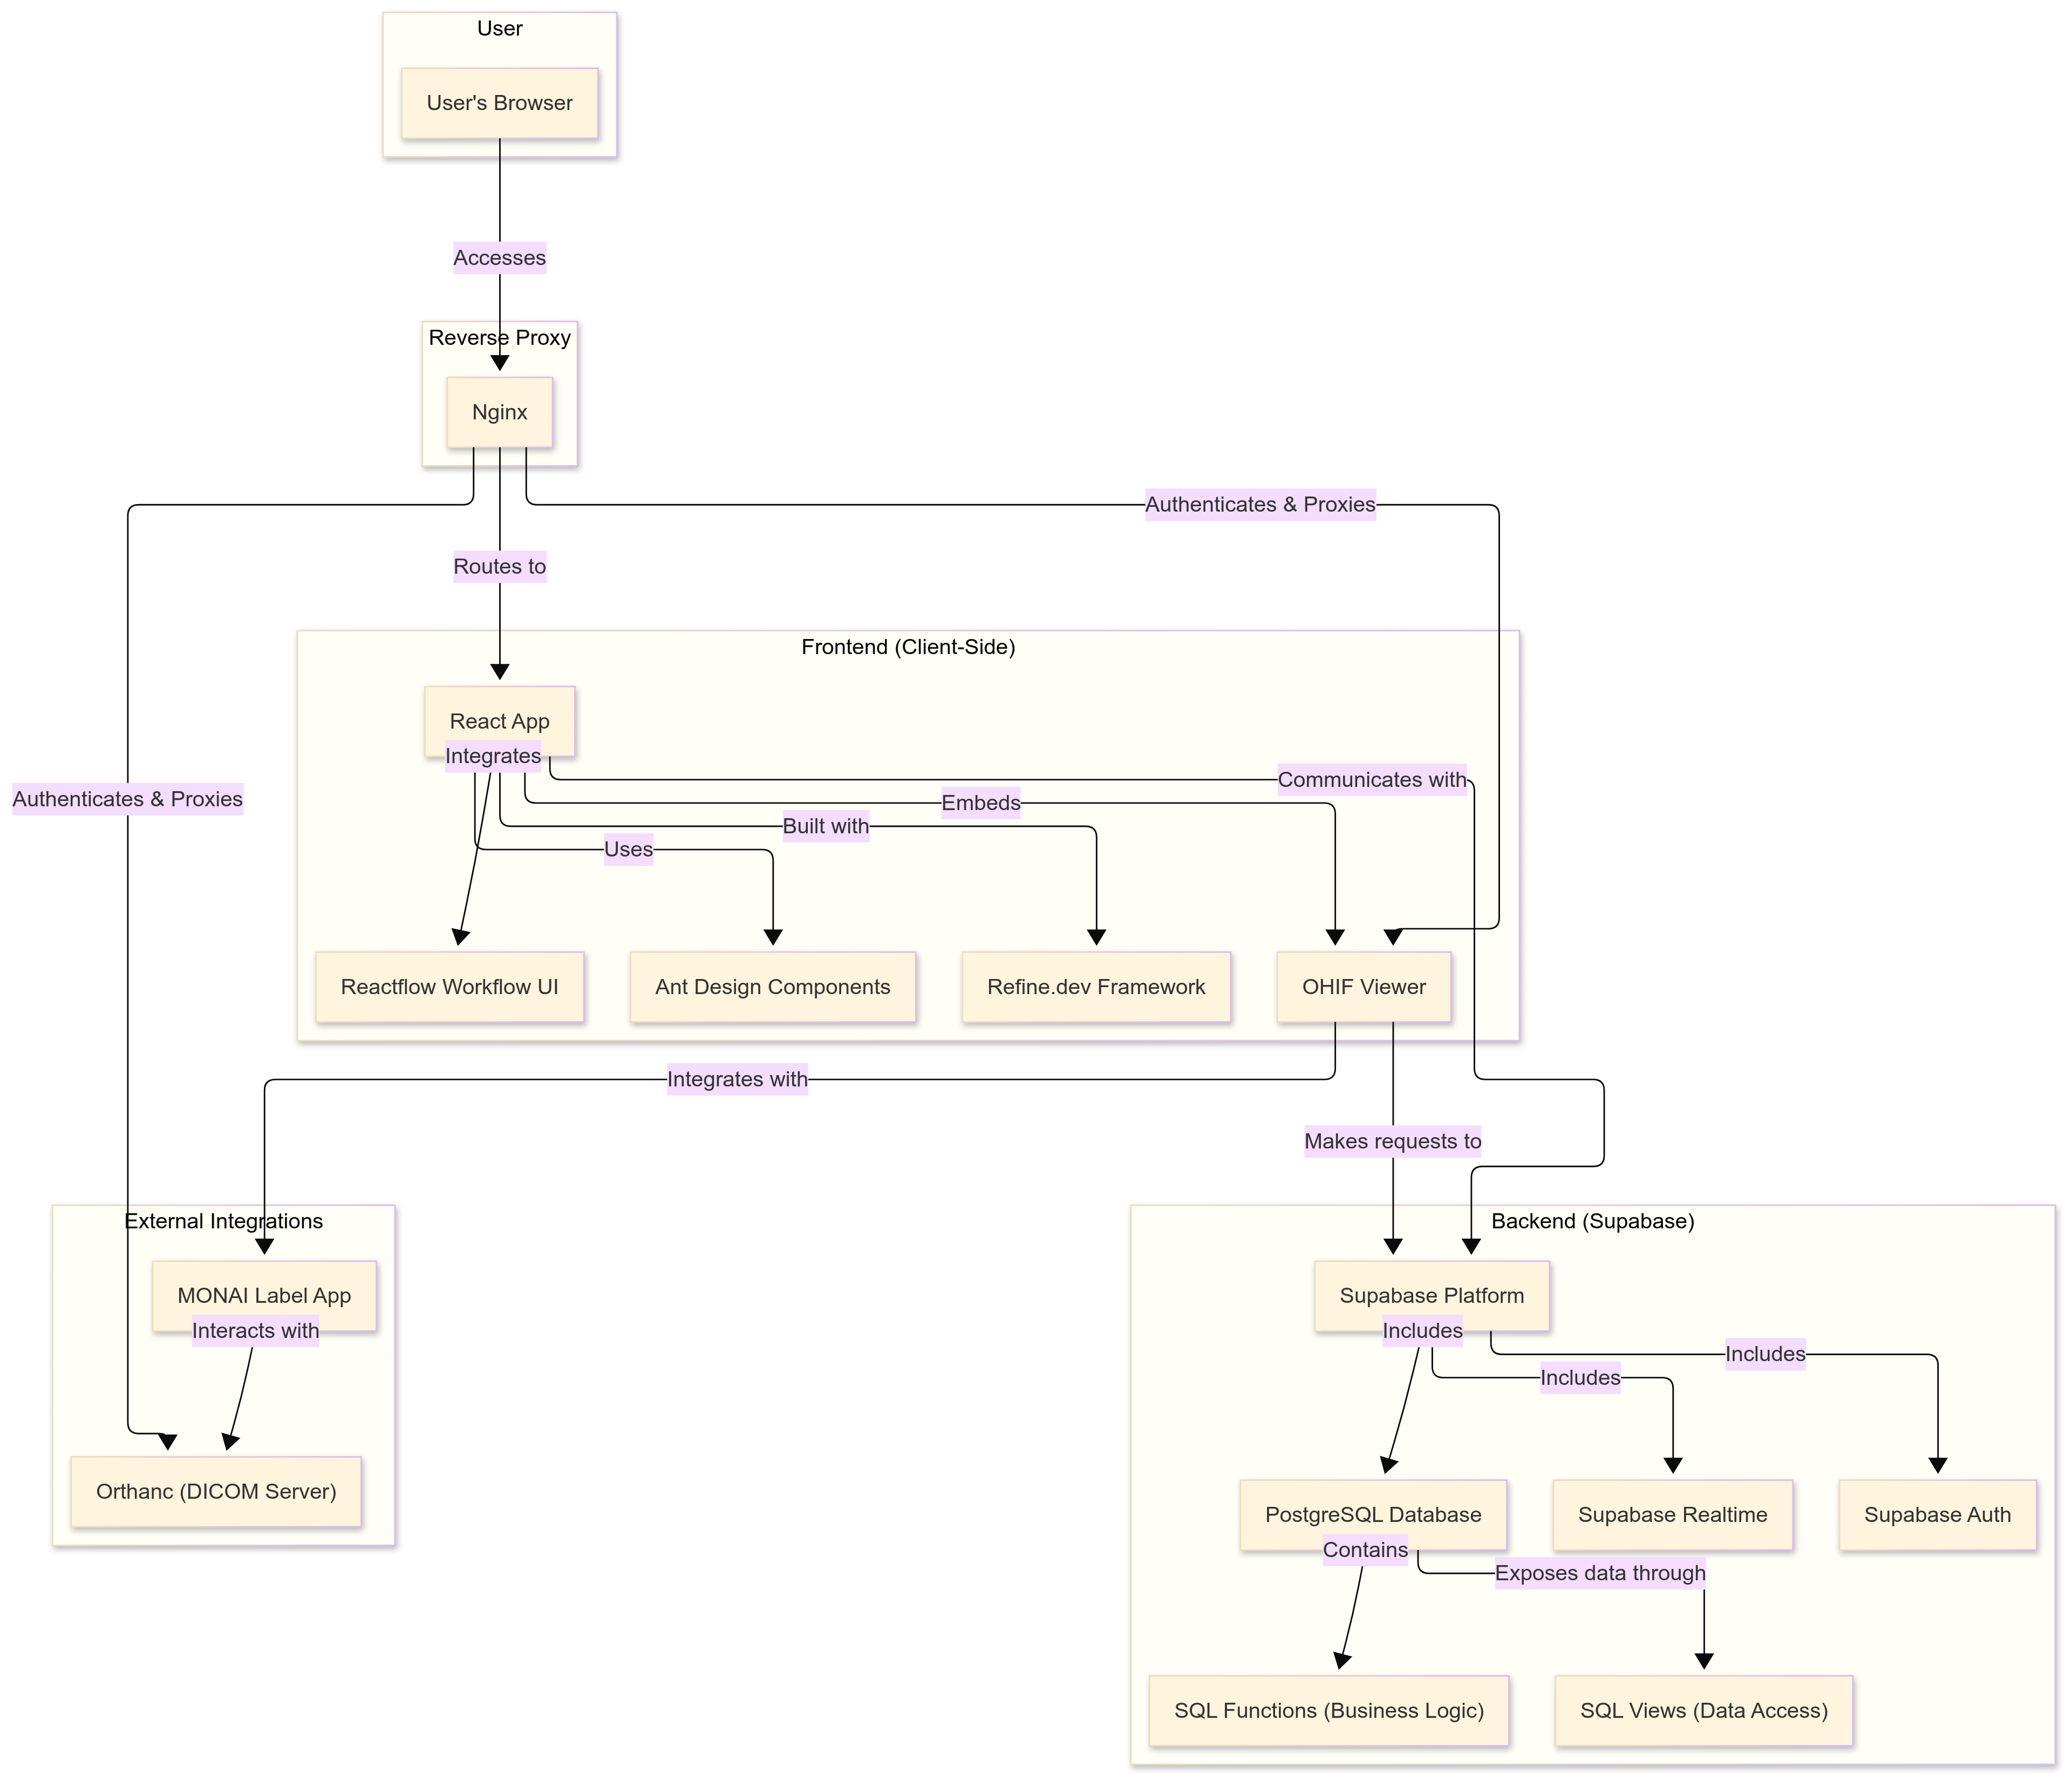
\includegraphics[width=0.95\textwidth]{content/resources/images/chap4-system-design/system-architecture.png}
\caption{Complete System Architecture - The intelligent medical annotation system architecture showing the comprehensive flow from user interaction through the Nginx reverse proxy to the React frontend, which integrates with multiple backend services including Supabase for real-time data management, OHIF Viewer for medical image visualization, and external services (MONAI Label and Orthanc DICOM Server) for AI assistance and medical data storage.}
\label{fig:system-architecture}
\end{figure}

The system architecture demonstrates several key optimization principles: the Nginx reverse proxy provides load balancing and SSL termination, the React frontend enables responsive user interfaces with real-time updates, Supabase delivers managed database services with built-in authentication and real-time capabilities, while external integrations with MONAI Label and Orthanc ensure specialized AI processing and DICOM compliance without adding complexity to the core system. This architectural approach maximizes performance while minimizing operational overhead.

\subsection{Component Interaction Design}

The system components interact through well-defined interfaces that ensure loose coupling while maintaining functional coherence and data consistency.

\textbf{API Gateway Pattern:} A centralized API gateway manages all external communication to the system, providing authentication, authorization, rate limiting, and request routing. This pattern simplifies client integration and enables consistent security policy enforcement across all services.

\textbf{Database per Service:} Each microservice maintains its own database instance optimized for its specific data access patterns and performance requirements. This approach prevents database-level coupling while enabling service-specific optimization.

\textbf{Event-Driven Integration:} Services publish and subscribe to domain events that enable loose coupling and asynchronous processing. This pattern is particularly important for workflow state transitions and long-running AI processing tasks.

\textbf{Circuit Breaker Pattern:} The system implements circuit breaker patterns to handle service failures gracefully, preventing cascade failures and maintaining system stability during partial outages.

\subsection{Security and Access Control Architecture}

Security is implemented as a cross-cutting concern that protects both data and system functionality while enabling appropriate access for authorized users.

\textbf{Zero Trust Security Model:} The system implements a zero trust security model where every request is authenticated and authorized regardless of its source \cite{rose2020zero}. This approach ensures comprehensive security protection in distributed and cloud deployment scenarios.

\textbf{Attribute-Based Access Control (ABAC):} Beyond role-based permissions, the system implements attribute-based access control that considers contextual factors such as data sensitivity, project membership, and temporal constraints when making access decisions \cite{hu2014guide}.

\textbf{Data Encryption and Protection:} All data is encrypted both in transit and at rest using industry-standard encryption algorithms. The system implements key management practices that ensure encryption keys are properly secured and rotated according to healthcare security standards.

\section{Workflow Management Module Design}

\subsection{Database Schema and Data Architecture}

The workflow management module utilizes a carefully designed PostgreSQL database schema that efficiently supports complex medical annotation workflows while maintaining data integrity and performance.

\textbf{Core Entity Design:}

\begin{table}[htbp]
\centering
\caption{Core Database Entities and Relationships}
\label{tab:database-entities}
\begin{tabular}{|p{3cm}|p{4cm}|p{7cm}|}
\hline
\textbf{Entity} & \textbf{Primary Purpose} & \textbf{Key Relationships} \\
\hline
Projects & Project organization and configuration & Has many workflows, tasks, and members \\
\hline
Workflows & Workflow definition and orchestration & Belongs to project, has many stages and tasks \\
\hline
Workflow Stages & Individual workflow steps & Belongs to workflow, defines transitions \\
\hline
Tasks & Individual annotation work items & Belongs to project, progresses through stages \\
\hline
Task Assignments & User-specific work assignments & Links tasks to users at specific stages \\
\hline
Users & System user management & Has roles and project memberships \\
\hline
Annotations & Annotation results and metadata & Belongs to task assignments \\
\hline
\end{tabular}
\end{table}

\textbf{Workflow State Management:} The system implements a sophisticated state machine that tracks task progression through workflow stages. State transitions are implemented as atomic database operations that ensure consistency even in high-concurrency scenarios.

\textbf{Audit Trail Implementation:} All workflow operations are logged in comprehensive audit tables that track user actions, state changes, and system events. This audit trail supports compliance requirements and enables detailed workflow analysis and optimization.

\subsection{Workflow Engine Implementation}

The workflow engine represents the core business logic component that orchestrates annotation workflows according to defined rules and policies.

\textbf{Rule-Based Workflow Processing:} The engine implements a rule-based processing system that evaluates workflow transitions based on configurable rules. This approach enables complex workflow scenarios such as consensus building, quality control checkpoints, and conditional routing.

\textbf{Stage Type Implementation:} The system supports multiple workflow stage types, each with specific behaviors and requirements:

\begin{itemize}
    \item \textit{START:} Initial workflow entry point with automatic progression
    \item \textit{ANNOTATE:} Manual annotation stages requiring user interaction
    \item \textit{REVIEW:} Quality control stages with approval/rejection decisions
    \item \textit{CONSENSUS:} Multi-annotator stages requiring agreement mechanisms
    \item \textit{MITL (Model-in-the-Loop):} AI-assisted stages with automatic processing
    \item \textit{ROUTER:} Conditional routing stages based on configurable criteria
    \item \textit{SUCCESS:} Workflow completion stages with final processing
\end{itemize}

\textbf{Concurrent Processing Support:} The workflow engine supports concurrent processing of multiple tasks and parallel execution of workflow stages where appropriate. This capability significantly improves overall system throughput for large annotation projects.

\subsection{Task Assignment and Routing Logic}

The task assignment system implements intelligent routing that considers multiple factors to optimize annotation efficiency and quality.

\textbf{Competency-Based Assignment:} The system maintains competency profiles for users that define their qualifications for different types of annotation tasks. Assignment algorithms consider these profiles to ensure tasks are routed to appropriately qualified annotators.

\textbf{Workload Balancing:} The assignment system implements sophisticated workload balancing that considers current user workload, task complexity, and deadline requirements. This balancing helps prevent annotator overload while maintaining consistent progress across all active projects.

\textbf{Priority-Based Routing:} Tasks can be assigned different priority levels that influence routing decisions. High-priority tasks may be routed to senior annotators or processed ahead of normal workflow queues.

\textbf{Consensus Building Logic:} For tasks requiring consensus, the system implements configurable consensus mechanisms that can require agreement from multiple annotators or use majority voting approaches depending on project requirements.

\subsection{Notification and Communication System}

The notification system ensures that users receive timely information about task assignments, workflow events, and collaboration opportunities.

\textbf{Multi-Channel Notification Delivery:} The system supports multiple notification channels including in-application notifications, email alerts, and mobile push notifications. Users can configure their notification preferences based on their role and work patterns.

\textbf{Real-Time Communication Features:} The system includes real-time communication features that enable immediate consultation and collaboration between annotators. These features include instant messaging, screen sharing, and collaborative annotation sessions.

\textbf{Escalation and Timeout Management:} The notification system implements escalation procedures for overdue tasks and automatic timeout management for tasks that exceed defined time limits. These features help maintain workflow momentum and identify potential bottlenecks.

\section{Annotation Interface Module Design}

\subsection{OHIF Integration and Customization}

The annotation interface builds upon the OHIF Viewer platform, extending it with specialized features required for intelligent medical annotation workflows.

\textbf{OHIF Viewer Foundation:} The system utilizes OHIF Viewer 3.x as the foundational medical imaging platform, providing robust DICOM support, high-performance image rendering, and extensible architecture. This foundation ensures compatibility with existing medical imaging infrastructure while providing a familiar interface for medical professionals.

\textbf{Custom Extension Development:} Several custom OHIF extensions have been developed to integrate workflow management, AI assistance, and collaborative features:

\begin{itemize}
    \item \textit{Workflow Integration Extension:} Connects the viewer to the workflow management system for task retrieval and status updates
    \item \textit{AI Assistance Extension:} Integrates MONAI Label capabilities directly into the annotation interface
    \item \textit{Collaboration Extension:} Enables real-time collaborative annotation and communication features
    \item \textit{Quality Control Extension:} Provides specialized tools for annotation review and validation
\end{itemize}

\textbf{Mode-Based Interface Configuration:} The system implements different interface modes optimized for specific workflows:

\begin{itemize}
    \item \textit{Annotation Mode:} Optimized for initial annotation tasks with AI assistance
    \item \textit{Review Mode:} Specialized for quality control and validation workflows
    \item \textit{Consensus Mode:} Designed for collaborative consensus-building sessions
    \item \textit{Training Mode:} Educational interface for training new annotators
\end{itemize}

\subsection{User Interaction Design and Experience}

The user interface is designed specifically for medical professionals, emphasizing efficiency, accuracy, and user satisfaction.

\textbf{Medical Professional-Centric Design:} The interface design follows established medical imaging conventions and incorporates feedback from practicing radiologists and medical technicians. This approach ensures that the system enhances rather than disrupts established clinical workflows.

\textbf{Adaptive Interface Layout:} The system supports adaptive interface layouts that automatically adjust based on screen size, user preferences, and task requirements. This adaptability ensures optimal user experience across different devices and work environments.

\textbf{Keyboard and Gesture Support:} The interface includes comprehensive keyboard shortcuts and gesture support that enable rapid navigation and annotation. These features are particularly important for experienced users who value efficiency and speed.

\textbf{Context-Sensitive Help:} The system provides context-sensitive help and guidance that assists users in understanding available features and completing complex annotation tasks. This support is particularly valuable for new users and complex annotation scenarios.

\subsection{Real-Time Collaboration Features}

The collaboration features enable multiple medical professionals to work together effectively on annotation tasks while maintaining annotation quality and consistency.

\textbf{Simultaneous Multi-User Annotation:} The system supports simultaneous annotation by multiple users on the same medical imaging study. Real-time synchronization ensures that all participants see the same view and can observe each other's annotations in real-time.

\textbf{Collaborative Annotation Tools:} Specialized tools enable collaborative annotation scenarios including shared pointer indicators, collaborative measurement tools, and group annotation sessions with voice communication integration.

\textbf{Conflict Resolution Mechanisms:} When multiple users annotate the same anatomical structures, the system provides conflict resolution mechanisms that help users reconcile differences and reach consensus on final annotations.

\textbf{Session Recording and Playback:} Collaboration sessions can be recorded for training purposes, quality control review, or documentation of complex annotation decisions. These recordings help preserve valuable medical knowledge and support continuous improvement.

\section{AI Assistance Module Design}

\subsection{MONAI Label Integration Architecture}

The AI assistance module integrates MONAI Label framework to provide state-of-the-art AI support for medical annotation tasks.

\textbf{MONAI Label Service Architecture:} The MONAI Label service is deployed as a containerized microservice that provides AI inference capabilities through RESTful APIs. This architecture enables scalable deployment and easy integration with the annotation interface.

\textbf{Model Management Framework:} The system implements a comprehensive model management framework that supports multiple AI models, model versioning, and dynamic model loading based on annotation requirements.

\textbf{Interactive Segmentation Pipeline:} The system implements an interactive segmentation pipeline that combines automated AI predictions with user guidance to produce high-quality annotations with minimal manual effort.

\subsection{AI Model Integration and Management}

The system supports integration of multiple AI models optimized for different medical imaging tasks and anatomical structures.

\textbf{Foundation Model Support:} The system integrates the SAM foundation model that provides comprehensive segmentation capabilities for over 127 anatomical structures across multiple medical imaging modalities.

\textbf{Specialized Model Integration:} In addition to foundation models, the system supports integration of specialized models optimized for specific anatomical regions or pathological conditions:

\begin{itemize}
    \item \textit{DeepEdit:} Interactive segmentation model for user-guided annotation
    \item \textit{Organ-Specific Models:} Specialized models for liver, lung, brain, and other organ systems
    \item \textit{Pathology Detection Models:} Models trained for specific pathological findings
    \item \textit{Custom Institutional Models:} Support for institution-specific model integration
\end{itemize}

\textbf{Model Performance Monitoring:} The system includes comprehensive model performance monitoring that tracks prediction accuracy, processing time, and user satisfaction metrics. This monitoring enables continuous model improvement and optimization.

\subsection{Interactive Segmentation Workflow}

The interactive segmentation workflow combines automated AI capabilities with expert guidance to achieve optimal annotation results.

\textbf{AI-First Annotation Approach:} The workflow begins with AI-generated preliminary annotations that provide a starting point for expert review and refinement. This approach significantly reduces manual annotation time while maintaining high quality standards.

\textbf{Progressive Refinement Interface:} Users can progressively refine AI predictions through various interaction methods including point clicks, boundary adjustments, and region corrections. The AI model adapts to user corrections in real-time, improving subsequent predictions.

\textbf{Uncertainty Visualization:} The system visualizes AI prediction uncertainty to help users focus their attention on areas where manual review is most beneficial. This feature enables efficient allocation of expert time and attention.

\textbf{Quality Assessment Integration:} Automated quality assessment tools evaluate annotation consistency and accuracy, providing real-time feedback to users and identifying potential areas for improvement.

\section{Data Management Module Design}

\subsection{DICOM Storage and Management}

The data management module provides comprehensive DICOM storage and management capabilities that ensure compatibility with existing medical imaging infrastructure.

\textbf{Orthanc PACS Integration:} The system utilizes Orthanc as the core DICOM storage platform, providing full DICOM compliance, DICOMweb protocol support, and seamless integration with existing hospital PACS systems.

\textbf{Scalable Storage Architecture:} The storage architecture supports both local and cloud-based storage backends, enabling flexible deployment options that accommodate different institutional requirements and constraints.

\textbf{Performance Optimization:} The system implements various performance optimization techniques including image caching, progressive loading, and intelligent prefetching to ensure optimal user experience even with large medical imaging datasets.

\subsection{Metadata Synchronization and Management}

Effective metadata management is crucial for efficient annotation workflows and system integration.

\textbf{Automatic Metadata Extraction:} The system automatically extracts and indexes DICOM metadata to enable efficient search, filtering, and organization of medical imaging studies. This metadata supports workflow routing and task assignment decisions.

\textbf{Cross-System Synchronization:} The system implements automatic synchronization mechanisms that keep annotation metadata synchronized across all system components while maintaining data consistency and integrity.

\textbf{Custom Metadata Support:} The system supports custom metadata fields that enable institutions to add project-specific information and annotation requirements without modifying core system functionality.

\subsection{Backup and Recovery Strategies}

Robust backup and recovery capabilities ensure data protection and business continuity for critical medical annotation workflows.

\textbf{Multi-Level Backup Strategy:} The system implements a multi-level backup strategy that includes real-time replication, scheduled backups, and long-term archival storage. This approach ensures data protection against various failure scenarios.

\textbf{Point-in-Time Recovery:} The system supports point-in-time recovery capabilities that enable restoration of data and annotations to specific timestamps. This capability is crucial for recovering from data corruption or accidental modifications.

\textbf{Disaster Recovery Planning:} Comprehensive disaster recovery procedures ensure that the system can be restored quickly in the event of major infrastructure failures or natural disasters.

\section{Technology Stack Selection and Justification}

\subsection{Frontend Technology Choices}

The frontend technology stack is selected to provide optimal user experience while ensuring maintainability and extensibility.

\textbf{React Framework Selection:} React is chosen as the primary frontend framework due to its excellent performance, large ecosystem, and strong community support. React's component-based architecture aligns well with the modular design requirements of medical imaging interfaces.

\textbf{Refine.dev Integration:} Refine.dev is selected as the rapid development framework for administrative interfaces due to its built-in support for CRUD operations, authentication, and real-time updates. This choice significantly accelerates development of workflow management interfaces.

\textbf{Ant Design Component Library:} Ant Design provides a comprehensive component library that ensures consistent user interface design and reduces development time. The library's medical and scientific components are particularly well-suited for healthcare applications.

\textbf{OHIF Viewer Platform:} OHIF Viewer is selected as the medical imaging foundation due to its proven track record in clinical environments, extensive DICOM support, and active development community focused on medical imaging requirements.

\subsection{Backend Technology Decisions}

The backend technology stack is selected to provide scalability, reliability, and integration capabilities required for healthcare applications.

\textbf{Supabase Platform Choice:} Supabase is selected as the backend platform due to its real-time capabilities, built-in authentication, and PostgreSQL foundation. These features provide excellent support for collaborative workflows and real-time annotation updates.

\textbf{PostgreSQL Database Selection:} PostgreSQL is chosen as the primary database due to its excellent performance with complex queries, strong consistency guarantees, and extensive JSON support that accommodates flexible annotation metadata requirements.

\textbf{Node.js Runtime Environment:} Node.js is selected for custom backend services due to its excellent performance for I/O-intensive operations and large ecosystem of medical imaging libraries.

\subsection{AI and Machine Learning Infrastructure}

The AI infrastructure is designed to provide high-performance model inference while maintaining flexibility for future model integration.

\textbf{MONAI Framework Selection:} MONAI is chosen as the primary AI framework due to its specific focus on medical imaging applications, comprehensive model library, and strong integration capabilities with medical imaging workflows.

\textbf{PyTorch Deep Learning Platform:} PyTorch is selected as the underlying deep learning platform due to its dynamic computation graphs, excellent debugging capabilities, and strong support in the medical imaging research community.

\textbf{Docker Containerization Strategy:} Docker containerization is used throughout the system to ensure consistent deployment across different environments and enable scalable infrastructure management.

\subsection{Infrastructure and Deployment Architecture}

The infrastructure architecture is designed to support both cloud and on-premises deployment while maintaining security and performance requirements.

\textbf{Nginx Reverse Proxy:} Nginx is selected as the reverse proxy and load balancer due to its excellent performance, robust security features, and extensive configuration capabilities required for medical imaging applications.

\textbf{Container Orchestration Strategy:} The system supports deployment using both Docker Compose for smaller installations and Kubernetes for large-scale deployments, providing flexibility for different institutional requirements.

\textbf{Monitoring and Observability:} Comprehensive monitoring and observability solutions are integrated to ensure system reliability and enable proactive maintenance and optimization. 